% Phase-1 Project Proposal
% Team: The Binary Guild
% Project: CheckMate
% Compile with pdfLaTeX.
% Member photos are intentionally left empty.
% To add them later, uncomment the corresponding \includegraphics line.

\documentclass[11pt,a4paper]{article}

\usepackage[a4paper,left=2.0cm,right=2.0cm,top=1.55cm,bottom=1.55cm]{geometry}
\usepackage[T1]{fontenc}
\usepackage{lmodern}
\usepackage{graphicx}
\usepackage{xcolor}
\usepackage{array}
\usepackage{tabularx}
\usepackage{ragged2e}
\usepackage{enumitem}
\usepackage{fancyhdr}
\usepackage{tikz}
\usetikzlibrary{positioning}
\usepackage{setspace}

% -------------------------------------------------
% COLOURS
% -------------------------------------------------

\definecolor{TitleBlue}{RGB}{61,103,154}

% -------------------------------------------------
% GENERAL SETTINGS
% -------------------------------------------------

\setlength{\parindent}{0pt}
\setlength{\parskip}{0pt}
\renewcommand{\arraystretch}{1.0}

\newcommand{\blueheading}[1]{%
    {\sffamily\color{TitleBlue}\fontsize{15}{18}\selectfont #1}%
}

\newcommand{\bluebigheading}[1]{%
    {\sffamily\bfseries\color{TitleBlue}\fontsize{16}{19}\selectfont #1}%
}

\newcommand{\instruction}[1]{%
    {\itshape\fontsize{10.5}{12.5}\selectfont #1}%
}

\newcommand{\answerbox}[2][3.0cm]{%
    \vspace{2pt}%
    \noindent
    \fbox{%
        \begin{minipage}[t]{\dimexpr\textwidth-2\fboxsep-2\fboxrule\relax}
            \vspace{1mm}%
            {\fontsize{9.2}{11}\selectfont\itshape #2}%
            \vspace{1mm}%
        \end{minipage}%
    }%
}

% -------------------------------------------------
% HEADER / FOOTER
% -------------------------------------------------

\pagestyle{fancy}
\fancyhf{}
\renewcommand{\headrulewidth}{0pt}
\renewcommand{\footrulewidth}{0pt}

\fancyhead[L]{%
    \sffamily\bfseries\itshape\fontsize{10.5}{12}\selectfont
    Btech(cse)    DSCPP-III-2026-T279
}

\fancyhead[R]{%
    \sffamily\bfseries\fontsize{10.5}{12}\selectfont
    PROJECT PROPOSAL
}

\fancyfoot[R]{%
    \itshape\fontsize{10}{12}\selectfont
    Page \thepage
}

\setlength{\headheight}{14pt}
\setlength{\headsep}{23pt}
\setlength{\footskip}{24pt}

% -------------------------------------------------
% PAGE 1
% -------------------------------------------------

\begin{document}

\vspace*{4mm}

\bluebigheading{PROJECT AND TEAM INFORMATION}

\vspace{13mm}

\blueheading{Project Title}

\vspace{1mm}
\answerbox[1.0cm]{CheckMate: Intelligent Chess Game Using Data Structures}

\vspace{13mm}

\blueheading{Student / Team Information}

\vspace{2mm}

% Three-member layout. Photos are intentionally left empty.

\noindent
\begin{tabularx}{\textwidth}{|>{\RaggedRight\arraybackslash}p{0.69\textwidth}|>{\RaggedRight\arraybackslash}X|}
\hline
\begin{minipage}[t]{\linewidth}
\vspace{1.5mm}
\textit{\textbf{Team Name:}}\\[-1mm]
\vspace{1.5mm}
\end{minipage}
&
\begin{minipage}[t]{\linewidth}
\vspace{1.5mm}
\textit{The Binary Guild}
\vspace{1.5mm}
\end{minipage}
\\
\hline

\begin{minipage}[t][3.25cm][t]{\linewidth}
\vspace{1.5mm}
\textbf{Team member 1 (Team Lead)}\\[-1mm]
\vspace{2.0cm}
\end{minipage}
&
\begin{minipage}[t][3.25cm][t]{\linewidth}
\vspace{1.5mm}
\textit{Salar, Arnav -- 2510010793}\\
\textit{2510010793@geu.ac.in}
\vspace{2mm}
% ADD MEMBER 1 PHOTO HERE:
 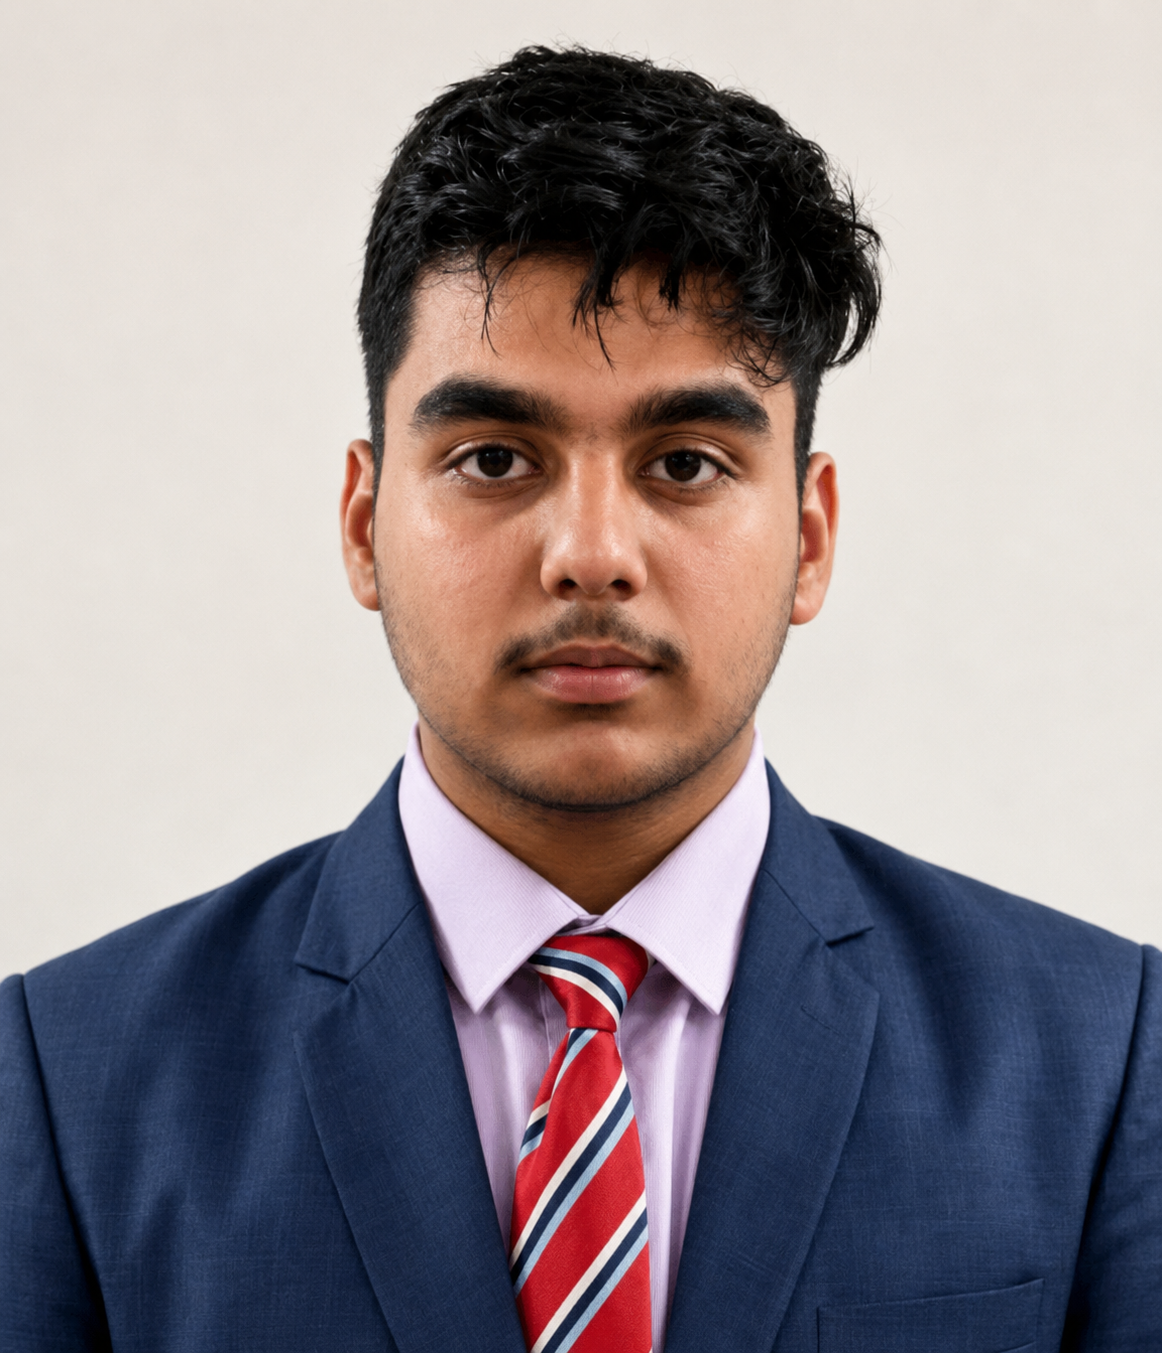
\includegraphics[width=3.0cm,height=1.5cm,keepaspectratio]{arnav.png}
\begin{figure}
    \centering
    \includegraphics[width=0.5\linewidth]{}
\begin{figure}
        \centering
        \includegraphics[width=0.5\linewidth]{}
        \caption{Enter Caption}
        \label{fig:placeholder}
    \end{figure}
        \caption{Enter Caption}
    \label{fig:placeholder}
\end{figure}
\end{minipage}
\\
\hline

\begin{minipage}[t][3.25cm][t]{\linewidth}
\vspace{1.5mm}
\textbf{Team member 2}\\[-1mm]
\vspace{2.0cm}
\end{minipage}
&
\begin{minipage}[t][3.25cm][t]{\linewidth}
\vspace{1.5mm}
\textit{Nishav -- 2510012485}\\
\textit{2510012485@geu.ac.in}
\vspace{2mm}
% ADD MEMBER 2 PHOTO HERE:

\includegraphics[width=3.0cm,height=1.5cm,keepaspectratio]{nishav.png}
\end{minipage}
\\
\hline

\begin{minipage}[t][3.25cm][t]{\linewidth}
\vspace{1.5mm}
\textbf{Team member 3}\\[-1mm]
\vspace{2.0cm}
\end{minipage}
&
\begin{minipage}[t][3.25cm][t]{\linewidth}
\vspace{1.5mm}
\textit{Painuly, Arush -- 2510011635}\\
\textit{2510011635@geu.ac.in}
\vspace{2mm}
% ADD MEMBER 3 PHOTO HERE:
 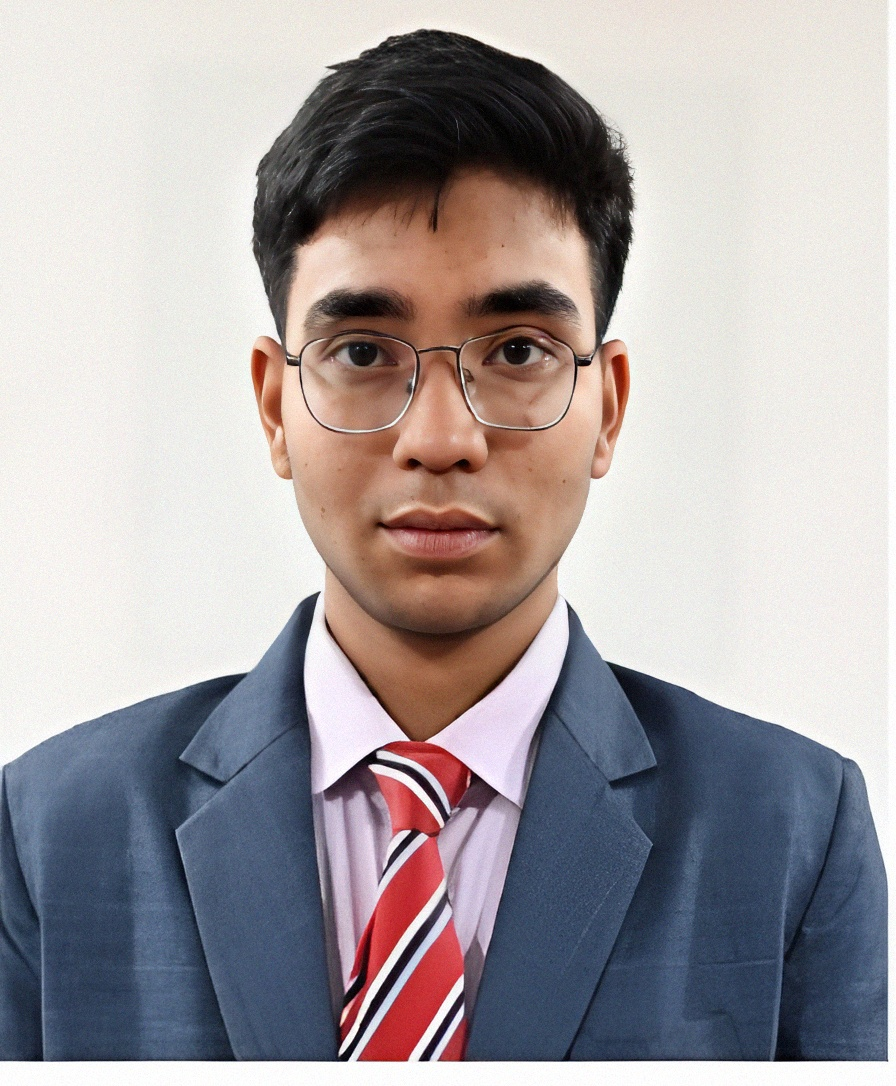
\includegraphics[width=3.0cm,height=1.5cm,keepaspectratio]{arush photo .png}
\end{minipage}
\\
\hline

\end{tabularx}

\newpage

% -------------------------------------------------
% PAGE 2
% -------------------------------------------------

\bluebigheading{PROPOSAL DESCRIPTION (10 pts)}

\vspace{12mm}

\blueheading{Motivation (1 pt)}

\vspace{1mm}
\answerbox[3.0cm]{
Chess is a strategy game that demonstrates Data Structures and Algorithms through board representation, move management, searching, and decision making. CheckMate will develop a functional chess game where DSA is a core part of the implementation.

The system will manage the board, legal moves, move history, undo operations, and game states using suitable structures. A basic computer opponent will use a game tree and Minimax search. The project will combine arrays, linked lists, stacks, queues, trees, hashing, searching, and sorting in one practical application.
}

\vspace{12mm}

\blueheading{State of the Art / Current solution (1 pt)}

\vspace{1mm}

\answerbox[2.75cm]{
Modern chess applications use chess engines to validate moves, evaluate positions, search possible game states, and select moves for computer players. They may also provide game records, timers, saving, and analysis.

In CheckMate, the core data structures and algorithms will be implemented manually. C will contain the DSA modules, while C++ will provide the main application and interaction layer. This keeps the project focused on understanding DSA internally.
}

\vspace{12mm}

\blueheading{Project Goals and Milestones (2 pts)}

\vspace{1mm}
\answerbox[3.15cm]{
The main goal is to develop a functional chess game that clearly demonstrates DSA concepts.

Initial milestones:
1. Represent the 8x8 board and implement legal moves.
2. Use a Linked List for move history and a Stack for undo.
3. Use a Queue for controlled event processing.
4. Implement hashing, searching, and sorting.
5. Build a move tree and basic Minimax opponent.
6. Integrate C DSA modules with the C++ application.
7. Add save/load and test complete games.
}

\vspace{12mm}

\blueheading{Project Approach (3 pts)}

\vspace{1mm}
\answerbox[3.05cm]{
C++ will be used for the main application and C for the core Data Structures and Algorithms. The board will use a two-dimensional array. A Linked List will store move history, a Stack will support undo, and a Queue will handle controlled event processing.

A tree will represent possible moves for game search. Minimax will provide the basic computer opponent. Hashing will support board-state lookup, while searching and sorting will assist move management. Standard C/C++ libraries and file handling will be used. The first version will be console-based so the DSA implementation remains the main focus.
}

\newpage

% -------------------------------------------------
% PAGE 3
% -------------------------------------------------

\blueheading{System Architecture (High Level Diagram)(2 pts)}

\vspace{1mm}
\answerbox[4.0cm]{
\begin{center}
\begin{tikzpicture}[
    node distance=0.55cm and 0.65cm,
    every node/.style={font=\small},
    box/.style={draw, rounded corners, minimum width=2.35cm, minimum height=0.58cm, align=center},
    arrow/.style={->, thick}
]

\node[box] (player) {Player /\\Game Input};
\node[box, right=of player] (cpp) {C++ Game\\Application};
\node[box, right=of cpp] (rules) {Chess Rules\\Engine};

\node[box, below=of cpp] (board) {Board Array\\(C)};
\node[box, below=of player] (stack) {Stack / Linked List\\(C)};
\node[box, below=of rules] (tree) {Move Tree /\\Minimax (C)};
\node[box, below=of board] (hash) {Hashing / Search\\(C)};

\draw[arrow] (player) -- (cpp);
\draw[arrow] (cpp) -- (rules);
\draw[arrow] (cpp) -- (board);
\draw[arrow] (cpp) -- (stack);
\draw[arrow] (rules) -- (tree);
\draw[arrow] (board) -- (hash);

\end{tikzpicture}
\end{center}
}

\vspace{12mm}

\blueheading{Project Outcome / Deliverables (1 pts)}

\vspace{1mm}
\answerbox[2.7cm]{
The project will deliver a functional chess game with two-player gameplay and a basic computer opponent. It will include board representation, legal move validation, move history, undo operations, game-state management, and basic game search.

Deliverables will include the C++ application, C-based DSA modules, move tree, Minimax opponent, hashing/search components, save/load functionality, test cases, documentation, and final demonstration.
}

\vspace{12mm}

\blueheading{Assumptions}

\vspace{6mm}
\answerbox[2.65cm]{
The project assumes standard chess rules and an 8x8 board. The initial version will implement essential legal moves, check, checkmate, and draw conditions required for demonstration. The computer opponent will be an educational implementation rather than a professional chess engine. Core DSA structures will be implemented manually in C, while C++ will handle the application layer and user interaction.
}

\vspace{12mm}

\blueheading{References}

\vspace{1mm}
\answerbox[2.65cm]{
1. Thomas H. Cormen et al., \textit{Introduction to Algorithms}, MIT Press.

2. Brian W. Kernighan and Dennis M. Ritchie, \textit{The C Programming Language}, Prentice Hall.

3. Bjarne Stroustrup, \textit{The C++ Programming Language}, Addison-Wesley.

4. Claude E. Shannon, ``Programming a Computer for Playing Chess'', Philosophical Magazine, 1950.

5. Course material and lecture notes on Data Structures and Algorithms.
}

\end{document}